\section{Data}\label{sec:sims}
\begin{figure}
\begin{center}
    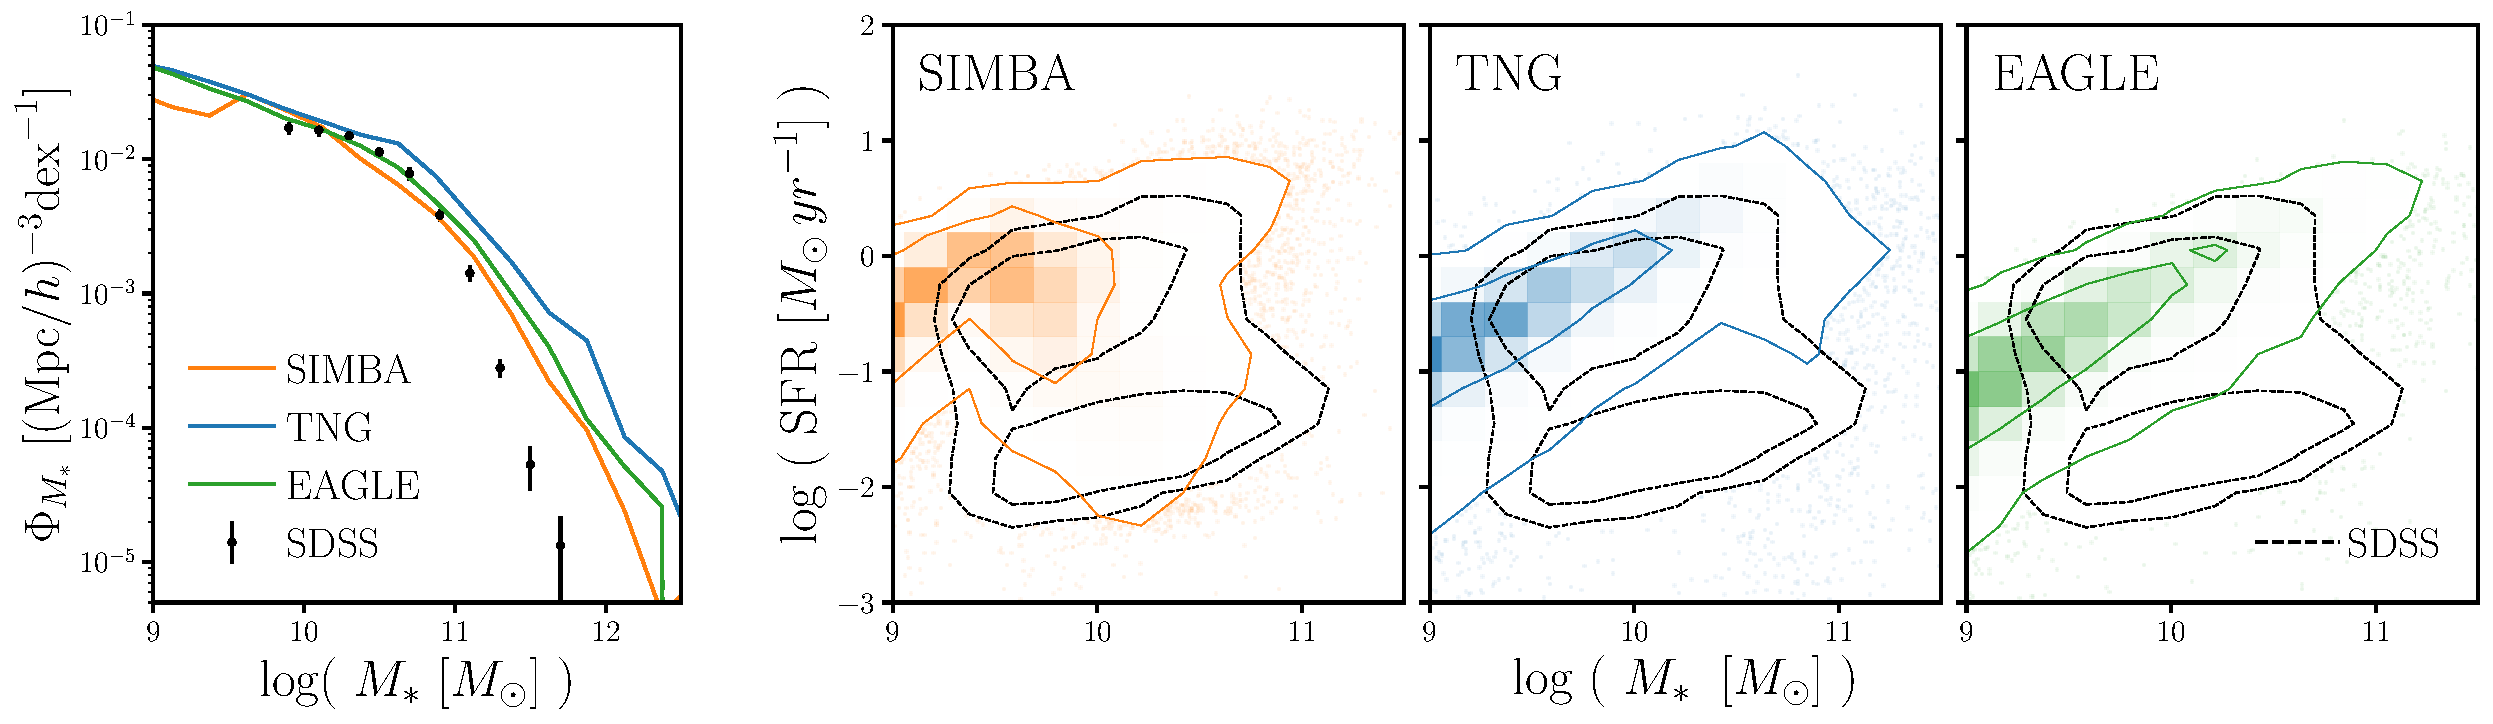
\includegraphics[width=\textwidth]{figs/smf_m_sfr.pdf}
    \caption{\label{fig:smf_msfr}
    The stellar mass functions of central galaxies, $\Phi^{\rm
    cen}_{M_*}$, of the SIMBA (orange) and TNG (blue) simulations compared to
    the SDSS $\Phi^{\rm cen}_{M_*}$. The uncertainties for the SDSS $\Phi^{\rm
    cen}_{M_*}$ are derived using jackknife resampling and SDSS centrals are
    identified using a halo-based group finder (Section~\ref{sec:obs}). For
    SIMBA and TNG galaxies, we calculate $M_*$ as the total stellar mass within
    the host halo, excluding contributions from any subhalos; centrals are
    classified based on their individual definition (Section~\ref{sec:tng}
    and~\ref{sec:simba}). {\color{red} should we include total SMF...?} 
    {\em The simulations and observations have loosely consistent $\Phi^{\rm
    cen}_{M_*}$.
    } 
    The $M_*-\sfr$ relation of central galaxies in SIMBA (orange), TNG (blue),
    and EAGLE (green) simulations and SDSS observations. \ch{describe where
    the M* and SFRs come from for everythign}. 
    The differences among the $M_*-\sfr$ relations demonstrate that the hydro
    simulations predict galaxy populations with significantly different
    physical properties. 
    }
\end{center}
\end{figure}

\subsection{SDSS DR7 Central Galaxies} \label{sec:obs} 
Throughout the paper we compare the simulations and models described below
to the observed SDSS central galaxy sample from the \cite{tinker2011} group
catalog. The group catalog, first, selects volume-limited sample of galaxies at
$z \approx 0.04$ with $M_r < -18$ and complete above $M_* > 10^{9.4}
h^{-2}M_\odot$ from the NYU Value-Added Galaxy
Catalog~\citep[VAGC;][]{blanton2005} of SDSS DR7~\citep{abazajian2009}. The
stellar masses are estimated using the $\mathtt{kcorrect}$
code~\citep{blanton2007a} assuming a~\cite{chabrier2003} initial mass
function. 

Central galaxies are then identified using a halo-based group finder that uses
the abundance matching ansatz to iteratively  assign halo masses to groups.
Every group contains one central galaxy, which by definition is the most
massive, and a group can contain $\ge0$ satellites. As with any group finder,
galaxies are misassigned due to projection effects and redshift space
distortions; however, the central galaxy sample has a purity of ${\sim}90\%$
and completeness of ${\sim}95\%$~\citep{tinker2018}. 

\subsection{Illustris TNG} \label{sec:tng}
\todo{describe what galaxy properties (SFH, ZH, etc) are available} 

\subsection{SIMBA} \label{sec:simba}
\todo{describe what galaxy properties (SFH, ZH, etc) are available} 

In Figure~\ref{fig:smf}, we compare the stellar mass function (SMF) of our SDSS
central galaxy sample along with central galaxy SMFs of the SIMBA (orange) and
TNG (blue) simulations. The uncertainties for the SDSS SMF are derived from
jackknife resampling. Although we present the SMFs for reference, we do not use
stellar masses throughout the paper since they are inconsistently defined among
simulations and observations. Instead, we compare between the simulations and
SDSS using luminosity, $M_r$, which we consistently forward model and measure
in the simulations. In these comparisons, we restrict ourselves to galaxies
brighter than $M_r < -20$, where our SDSS central galaxy sample is complete. 

instantaneous SFR=0 for $\sim11\%$ of SIMBA galaxies, $\sim13\%$ for TNG,
$\sim2\%$ for EAGLE

\subsection{Spectral Energy Distributions} \label{sec:sed}
\todo{describe how the SED is generated using the SFH and ZHs} 

\subsection{Forward Modeling Optical and UV photometry} \label{sec:fm} 

\cite{trayford2015} Figure 1.a. has a comparison without dust that's roughly
consistent with what we find for EAGLE



\begin{figure}
\begin{center}
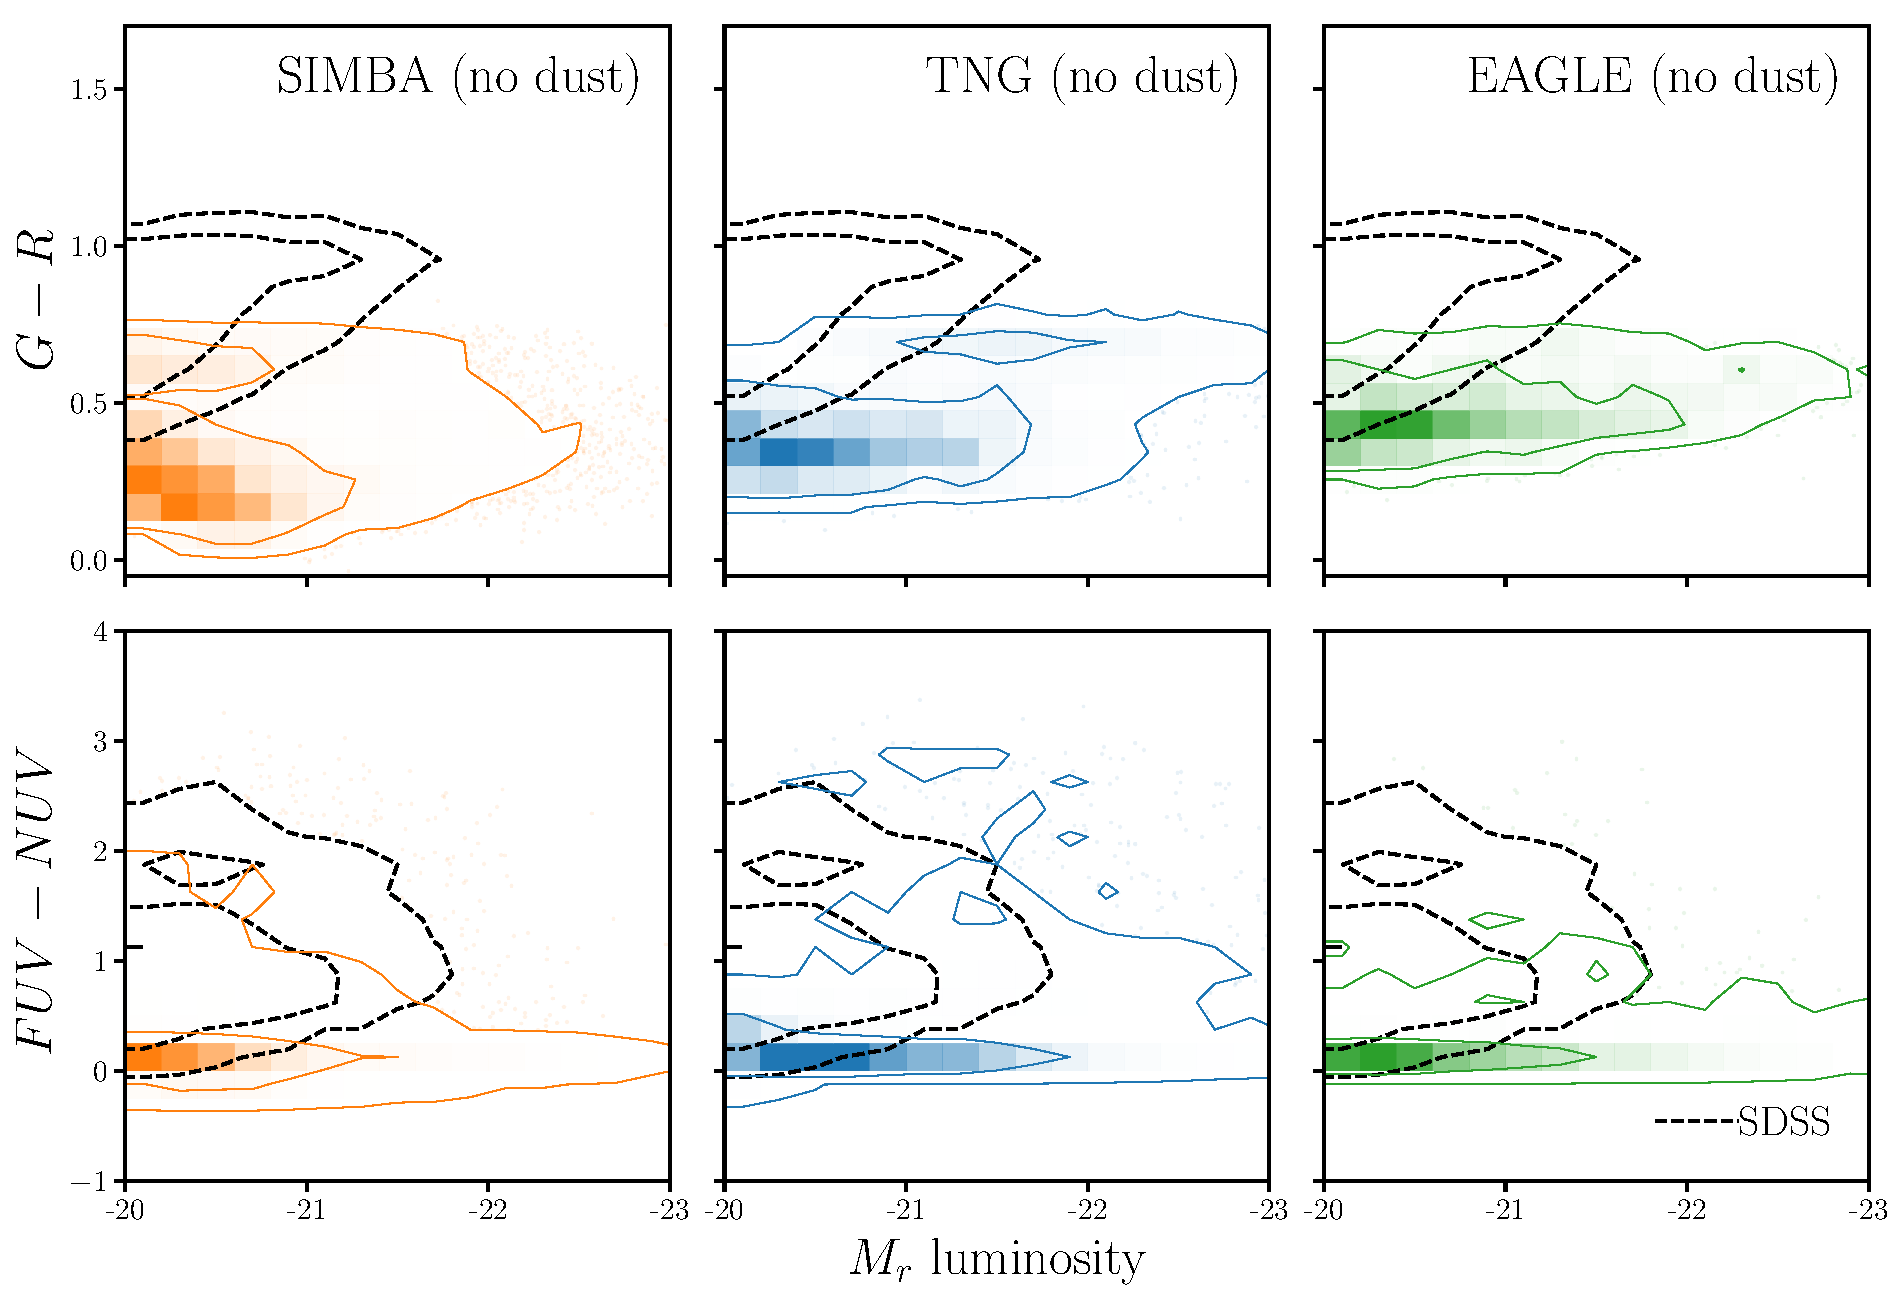
\includegraphics[width=0.9\textwidth]{figs/observables.pdf} 
    \caption{We present the distributions of the main observables used
    throughout the paper for SDSS (left), SIMBA (center), and TNG (right)
    centrals. We do {\em not} include any prescription for dust for the
    simulated galaxies. The top panels
    present the $G-R$ versus $M_r$ color magnitude relations while the bottom
    panels present the $FUV-NUV$ versus $M_r$ relations. The observables for
    the SIMBA and TNG simulated galaxies are derived using forward modeling and
    are therefore consistent with SDSS measurements (Section~\ref{sec:fm}). The
    contours for SIMBA and TNG do not include galaxies with SFR$=0$, which we
    mark separately in black. Despite similar SMFs,  {\em the simulations
    without any dust prescription show stark differences with observations in
    the color-magnitude observable-space.} 
    }
\label{fig:obs}
\end{center}
\end{figure}
